\begin{ccRefFunction}{compare_y}

Depending on which \cgal\ \ccHtmlNoLinksFrom{kernel} is used,
different versions of this global function are available. This is
described below.

%%%%%%%%%%%%%%%%%%%%%%%%%%%%%%%%%%%%%%%%%%%%%%
\paragraph{With the basic 2D and 3D Kernel} (see Chapter~\ref{chapter-kernel-23})

\ccFunction{Comparison_result compare_y(const Point_2<Kernel> &p,
                                        const Point_2<Kernel> &q);}
        {compares Cartesian $y$-coordinates of $p$ and $q$.}

\ccFunction{Comparison_result compare_y(const Point_3<Kernel> &p,
                                        const Point_3<Kernel> &q);}
        {compares Cartesian $y$-coordinates of $p$ and $q$.}

\begin{ccHtmlOnly}
<img border=0 src="fig/compare1.gif" align=middle alt="Comparison of the x 
or y coordinates of the (implicitly given) points in the boxes">
\end{ccHtmlOnly} 

\begin{ccTexOnly}
\begin{figure}[hb]
\centerline{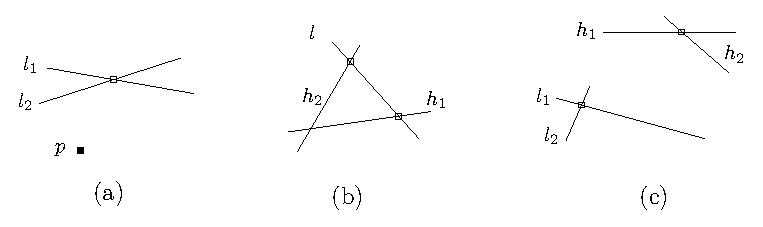
\includegraphics{Kernel_23_ref/fig/compare1}}
\caption{Comparison of the $x$ or $y$-coordinates of the (implicitly
given) points in the boxes.\label{fig-compare13}}
\end{figure} 
\end{ccTexOnly} 

\ccFunction{Comparison_result compare_y(const Point_2<Kernel> &p,
                                        const Line_2<Kernel> &l1,
                                        const Line_2<Kernel> &l2);}
        {compares the $y$-coordinates of $p$ and the \ccHtmlNoLinksFrom{intersection} of lines
         $l1$ and $l2$%
         \ccTexHtml{ (Figure~\ref{fig-compare13} (a))}{, see (a) in the figure 
         above}.}


\ccFunction{Comparison_result compare_y(const Line_2<Kernel> &l,
                                        const Line_2<Kernel> &h1,
                                        const Line_2<Kernel> &h2);}
        {compares the $y$-coordinates of the \ccHtmlNoLinksFrom{intersection} of line $l$
         with line $h1$ and with line $h2$%
         \ccTexHtml{ (Figure~\ref{fig-compare13} (b))}{, see (b) in the figure 
         above}.}


\ccFunction{Comparison_result compare_y(const Line_2<Kernel> &l1,
                                        const Line_2<Kernel> &l2,
                                        const Line_2<Kernel> &h1,
                                        const Line_2<Kernel> &h2);}
        {compares the $y$-coordinates of the \ccHtmlNoLinksFrom{intersection} of lines $l1$
         and $l2$ and  the \ccHtmlNoLinksFrom{intersection} of lines $h1$ and $h2$ 
         \ccTexHtml{ (Figure~\ref{fig-compare13} (c))}{, see (c) in the figure 
         above}.}

%%%%%%%%%%%%%%%%%%%%%%%%%%%%%%%%%%%%%%%%%%%%%%
\paragraph{With the 2D Circular Kernel} (see Chapter~\ref{chapter-circular-kernel}) 

\ccInclude{CGAL/global_functions_circular_kernel_2.h}

If this kernel is used, in addition to the function and the
combination of 2D types described above, another version of the function
is provided.

\ccFunction{Comparison_result 
  compare_y(const Circular_arc_point_2<CircularKernel> &p,
            const Circular_arc_point_2<CircularKernel> &q);}
{compares the $y$-coordinates of $p$ and $q$.}

\ccFunction{Comparison_result 
  compare_y(const Circular_arc_point_2<CircularKernel> &p,
            const Point_2<CircularKernel> &q);}
{compares the $y$-coordinates of $p$ and $q$.}

%%%%%%%%%%%%%%%%%%%%%%%%%%%%%%%%%%%%%%%%%%%%%%
\paragraph{With the 3D Spherical Kernel} (see Chapter~\ref{chapter-spherical-kernel}) 

\ccInclude{CGAL/global_functions_spherical_kernel_3.h}

If this kernel is used, in addition to the function and the
combination of 2D types described above, another version of the function
is provided.

\ccFunction{Comparison_result 
  compare_y(const Circular_arc_point_3<SphericalKernel> &p,
            const Circular_arc_point_3<SphericalKernel> &q);}
{compares the $y$-coordinates of $p$ and $q$.}

\ccFunction{Comparison_result 
  compare_y(const Circular_arc_point_3<SphericalKernel> &p,
            const Point_3<SphericalKernel> &q);}
{compares the $y$-coordinates of $p$ and $q$.}

%%%%%%%%%%%%%%%%%%%%%%%%%%%%%%%%%%%%%%%%%%%%%\ccSeeAlso
\ccRefIdfierPage{CGAL::compare_xy} \\
\ccRefIdfierPage{CGAL::compare_xyz} \\
\ccRefIdfierPage{CGAL::compare_x} \\
\ccRefIdfierPage{CGAL::compare_x_at_y} \\
\ccRefIdfierPage{CGAL::compare_yx} \\
\ccRefIdfierPage{CGAL::compare_y_at_x} \\
\ccRefIdfierPage{CGAL::compare_z} \\

\end{ccRefFunction}

